
%POUR COMPILER ASSURER VOUS D'AVOIR LE PAQUET SUIVANT POUR LINUX : TEXTLIVE-LATEXEXTRA

\documentclass[12pt,a4paper]{article}
\usepackage[utf8]{inputenc}
\usepackage[french]{babel}
\usepackage{amsmath}
\usepackage{amsfonts}
\usepackage{amssymb}
\usepackage {hyperref} % couleur du tableau
\usepackage{xcolor}	  % couleur du tableau
\usepackage{graphicx}
\usepackage{multirow} %Utilisation pour fusion case tableau%
\usepackage{colortbl} %COuleur Tableau%
\usepackage{fancyhdr}
\usepackage{times}
\usepackage[final]{pdfpages} 
%\usepackage[left=4cm,right=3cm,top=2cm,bottom=2.5cm]{geometry} %FUCKIN MARGE DE PETIT
\usepackage{setspace}
\definecolor{vert}{rgb}{0.1,0.6,0.1}
\usepackage{hyperref}                 
 \hypersetup{
    hyperfigures = true,
    colorlinks = true,
    linkcolor=black
    }
%\setstretch{1,5} % FUCKING INTERLIGNE DE PETIT
\author{Francois}
\sloppy

\title{Cahier des charges}

\renewcommand{\headrulewidth}{0.4pt}
\renewcommand{\footrulewidth}{0.4pt}
\fancyhead[L]{Info Spé}
\fancyhead[R]{Epita 2019}
\fancyfoot[L]{Facificator}

 \pagestyle{fancy}

\begin{document}

%Page de garde%


\begin{titlepage}


\flushright 
\includegraphics[scale=.15]{Pictures/EPITA_LOGO_DEF.png}
\flushright Promo 2019



\begin{center}


\hspace{1.5cm}
{\Huge Facificator}
\newline
\newline
\newline
\newline
\newline
%\includegraphics[scale=.35]{}
%Ici Logo

\end{center}
\begin{center}

%\vspace{0.7cm}
\end{center}
\begin{Large}
\begin{center}
Dexemple François, Luiggi Tristan, 
Ngo Jean-François, Utard Yannick  \end{center}
\end{Large}
\vspace{.5cm}
\begin{center}
\begin{large}
7 Decembre 2015
\end{large}
\end{center}

\noindent
\newline
\newline
\textit{Nom du groupe :} D.U.N.L. Studio \newline 
\textit{Chef de projet :} Dexemple François \newline
\end{titlepage}
\newpage

%% ICI sommaire %%
\newpage
\tableofcontents

%% Debut Document%%
\newpage
\section{Introduction}
Ce document est un rapport de projet et a pour but de présenter le logiciel Facificator après 13 semaines de travail sur ce dernier. Un logiciel réalisé par D.U.N.L Studio. Pour rappel, le logiciel réalisé est un logiciel de reconnaissance faciale développé en langage C, sous un environnement Unix. Celui-ci comporte plusieurs fonctionnalités telles que la reconnaissance faciale notamment.
Malgré la charge de travail conséquente, nous avons tenté tant bien que mal de tenir les objectifs fixés que vous pouvez retrouver dans ce rapport. Ainsi, ce projet nous a permis d'apprendre à coder en C grâce aux cours de programmation et aux travaux pratiques d'Epita. Mais également grâce à de nombreux tutoriels sur internet, qui nous ont permis de nous familiariser avec ce langage. Ce projet nous a également appris et fait découvrir la programmation événementielle avec le GTK.
Afin de réaliser ce projet de reconnaissance faciale, nous nous sommes basés sur la méthode de Viola et Jones publié en 2001.


\newpage

\section{Groupes}
\subsection{François Dexemple}
J'ai toujours aimé bidouiller les ordinateurs que ce soit sous Windows ou Linux, ou encore au niveau matériel. Par contre je n'ai jamais réellement touché à un langage de programmation à part ce que nous avons fait en C\# l'année dernière.
Je suis repartis cette année pour faire ce nouveau projet qui est peut être moins amusant à faire mais tout aussi intéressant. Pour ce projet je me suis remis avec Yannick, avec lequel je m'étais très bien entendu lors du projet de l'année dernière et deux autres anciens camarades de classe.\\
Étant très curieux à tout ce qui touche l'informatique j'apprends relativement vite les nouvelles choses qui m'intéressent. C'est donc avec enthousiasme que je commence ce projet. Pour ce projet je me suis porté volontaire pour faire la base de données car je suis en train de faire en parallèle une application androïd qui utilise une base SQLite, c'était donc un moyen de m'entrainer et de commencer assez vite à travailler puisque je connaissais déjà les bases. De plus, connaissant déjà très l'environnement Linux et git, grâce au projet de l'année dernière, j'ai pu commencer très vite 

\subsection{Tristan Luiggi}
Etant passionné d'informatique depuis l'enfance, intégrer l'EPITA était un choix évident lors de mon orientation en Terminale. Ainsi après une année passer des cette école j'ai pu commencer à apprendre quelques langages et me lancer dans des projets. Ces projet me permettent de me confronté a ce que pourrait être mon future métier d'ingénieur et d'améliorer plusieurs conpetances avec celui ci tel aue le travail d'equipe ou encore l'autonomie.
Le projet de l'année de SUP imposait peu de contrainte et donnait un accèe à un environnement de devellopement assez fourni, cette année nous âssons à la vitesse superieur avec l'arrivé de Linux et du language C. De plus la reconnaissance faciale nous oblige à abordé des notions totalement nouvelles. ce projet estun reel defis qui nous rendera plus autonome et competent à l'aboutissment.

\newpage

\subsection{Jean-François Ngo}
Depuis tout jeune, l'informatique a toujours été un domaine qui m'intéressait fortement même si je ne saurai expliquer précisément pourquoi. C'est pourquoi j'ai décidé d'intégrer une école comme Epita qui propose une formation dans ce sens. Après une première année ponctué par l'apprentissage d'un nouveau langage, le C\#, et la mise en pratique de ce langage dans un projet de réalisation d'un jeu vidéo qui a permis d'acquérir de nombreuses compétences et connaissances. Une deuxième année commence avec un nouveau projet à réaliser dans un nouveau langage qu'est le C, sous Linux. Ce projet, bien plus compliqué que celui de l'année dernière pour moi, est un nouveau défi qui nous oblige à énormément lire afin de comprendre comment marche la reconnaissance faciale, qui constitue un énorme travail en amont avant de commencer la programmation même par rapport au projet de l'année dernière. De plus, tout comme le projet de l'année dernière, je pense que ce projet me permettra de me plonger dans un travail d'équipe, de groupe, ce qui je pense m'attend dans ma future vie d'ingénieur.

\subsection{Yannick Utard}
Comme l'année dernière nous revoilà sur un nouveau projet en informatique. L'an dernier, il s'agissait d'un jeu vidéo, ce qui était un sujet très attrayant pour tout amateur en informatique. Le sujet de cette année était à première vue moins ludique, cependant il s'est révélé être très intéressant. Je n'avais jusqu'à présent jamais traité d'image de cette façon, mis à part lors d'un TP de C\# en SUP. De plus le C est un nouveau langage mais j'ai réussi à m'adapter rapidement grâce aux tutoriels sur internet et aux TPs de l'école; afin de progresser dans ce projet. 
Dans l'équipe, le D.U.N.L Studio, il y a une bonne ambiance étant donné que nous nous connaissons depuis la SUP et que j'ai travaillé sur le projet de l'an dernier avec François. Le projet avance donc dans la bonne humeur même si nous avons parfois eu du mal avec la gestion du temps car le travail est assez conséquent. Enfin, je pense que nous avons atteint nos objectifs pour cette première soutenance et nous ne sommes pas prêts de nous arrêter là !

\newpage
 
Le projet, réalisé par un groupe de quatre personnes sur une durée d'environ 13 semaines, est un logiciel de reconnaissance faciale. Le logiciel devra permettre à partir d'une photo de groupe d'identifier les personnes présentes sur la photo (Par exemple, pour une photo de classe, le logiciel devra être en mesure d'indiquer les personnes présentes sur la photo mais aussi de déterminer les absents). C'est un projet qui s'articule sur deux axes, l'apprentissage d'une base de visage à partir de photos d'identité et l'extraction des visages présents sur une photo de groupe comme dit précédemment. Ainsi, le logiciel final devra permettre de charger un ensemble de visages associées avec le nom de la personne correspondante pour construire la base de données, elle devra permettre d'ajouter de nouveaux visages ou de corriger les informations associées à ceux-ci également, mais elle permettra aussi de charger une photo de groupe et d'obtenir la liste des présentes sur la photo.

Ce projet sera développé sous Linux et sera codé en C uniquement (norme C99). Avec l'aide de toutes les bibliothèques disponibles ou directement installables sur le rack de l'école via les paquets, en particulier la bibliothèque SDL et ses composants pour le chargement des images et la bibliothèque GTK pour l'interface graphique. 

\newpage
\section{Nature et but du projet}
\subsection{Qu'est-ce que ?}
C'est un logiciel de recherche de personnes présentes sur une photo. A partir d'une photo le logiciel vous donnera la liste des personnes présentes sur la photo et se trouvant dans sa base de données.

\subsection{Principe}
L'utilisation du logiciel se découpe en deux parties : dans un premier temps l'utilisateur va remplir la base de données de visages dont seront extraites les informations pertinentes pour l'identification des personnes ; une fois la base remplie, le logiciel permettra à partir d'une photo de trouver la liste des personnes présentes.

Le logiciel devra également permettre de gérer la base en fournissant des opérations d'ajout, de suppression ou de correction des personnes enregistrées dans la base.

\subsection{Règles à respecter}

Pour que le développement de ce projet se passe le mieux possible, nous allons respecter les règles de programmations suivantes :

Pour le code :
\newline
- Indentation des fonctions obligatoire.
\newline
- Les noms de fonctions, variables, constantes et macros devront être en anglais.
\newline
- Établir un découpage correct et cohérent du code en plusieurs fichiers avec les fichiers d'en-têtes correspondant.
\newline
- 80 caractères par ligne.
\newline
- Pas d'espace en fin de ligne dans les fichiers .c et .h.
\newline
- Aucun warning à la compilation sur votre code (les seuls warning tolérés sont ceux produits par le code des bibliothèques utilisées.)


Pour le projet :
\newline
- Votre projet devra disposer d'un Makefile utilisable à l'école et sans modification. Celui-ci doit être compatible avec GNU Make.
\newline
- Votre Makefile devra compiler votre projet par défaut (appel à make sans paramètre ou avec all).
\newline
- Votre Makefile devra contenir une règle clean pour effacer tous les produits de la compilation.
\newline
- Vous pouvez utiliser indifféremment gcc ou clang pour compiler.
\newline
- Le code devra compiler avec les options suivantes : -Wall -Wextra -std=c99 -pedantic -03.
\newline
- Un fichier README, en anglais, qui explique comment compiler et utiliser votre projet.
\newline
- Un fichier AUTHORS listant les membres du projet, un par ligne sous la forme :
\newline
* login (NOM Prénom)

\section{Objectifs détaillés}
\subsection{Soutenance 1}
\subsubsection{Traitement d'un visage :}
- Détection du visage sur une photo d'identité (ou assimilée).
\newline
- Pré-traitement pour accentuer les caractéristiques intéressantes.
\newline
- Détection des éléments clefs pour l'analyse.
\newline
- Construction de la représentation caractéristique d'un visage.
\newline
- Option avancée : détection et découpage des visages dans une photo de groupe.

\subsubsection{Construction d'une base de données de caractéristiques de visage avec les noms associés :}
- Opérations de maintenance (ajout, suppression et modification).
\newline
- Ajouts en masse de visage dans la base (mode batch).
\newline
- Recherche d'une personne à partir d'un visage seul (photo d'identité ou visage extrait d'une photo de groupe.)

\subsection{Soutenance finale}
\subsubsection{Extraction de la liste des personnes :}
- Chargement et pré-traitement d'une photo de groupe.
\newline
- Finalisation de la détection et du découpage des visages dans une photo de groupe.
\newline
- Recherche des visages dans la base (identification par le nom associé d'un visage).

\subsubsection{Interface utilisateur permettant d'effectuer toutes les opérations, notamment :}
- Gestion complète de la base de données.
\newline
- Identification de visage(s) sur photo (individuelle ou de groupe).
\newline
- Comparaison entre deux visages.

\newpage
\section{Les tâches effectuées}
\subsection{Tableau récapitulatif}

\begin{tabular}{|c|c|c|c|c|}
\hline 
 & François & Tristan & Jean-François & Yannick \\ 
\hline 
Conversion d'une image & & & & \\ 
en niveau de gris & • & • & • & 100\% \\ 
\hline 
Conversion en image intégrale & • & • & • & 100\% \\ 
\hline 
Base de données & 100\% & • & • & • \\ 
\hline 
Interface graphique & 70\% & • & 30\% & • \\ 
\hline 
Adaboost & • & •  & • & 100\% \\ 
\hline 
Caractéristiques & • & • & • & 100\%  \\  
\hline
Détection & • & • & • & 100\%  \\  
\hline  
Reconnaissance & • & 100\% & • & •  \\  
\hline 
\end{tabular} 

\newpage
\subsection{Le traitement d'image}
Le traitement d'image est l'élément essentiel de ce projet en C. Il a été très important pour nous de directement nous informer le traitement des pixels d' une image être a l'aise sur ce projet ensuite. Pour charger une image, récupérer ses pixels ou encore l'afficher nous utilisons la bibliothèque SDL.

\vspace{0.8cm}
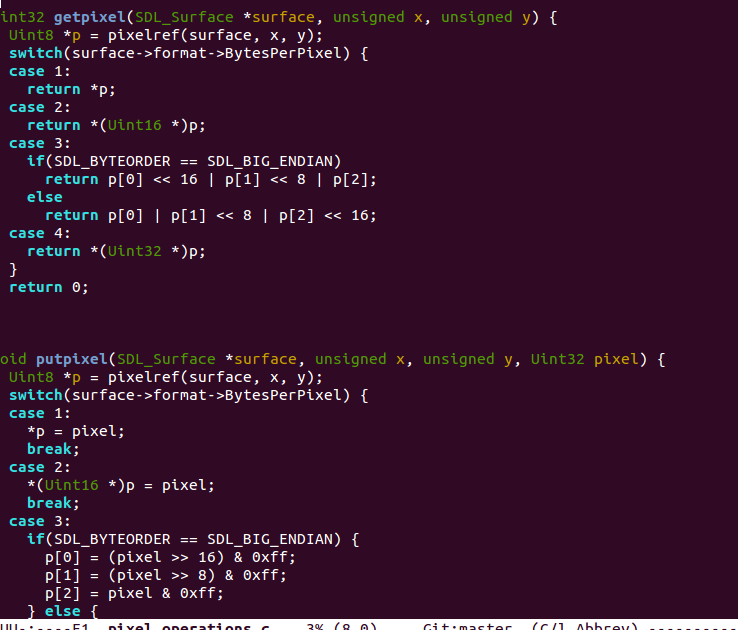
\includegraphics[scale=.5]{Pictures/sdl.png}
\vspace{0.8cm}

\newpage
Tout le traitement d'image se situe dans notre fichier pixel\_operations.c. Pour simplifier notre code, nous avons créés plusieurs structures en C dans le fichier types.h et quelques méthodes (d'allocation en particulier) pour ces structures dans types.c.
Par exemple, la structure training\_image\_t sert d'exemple d'apprentissage pour Adaboost (méthode de boosting, voir page...). Cette structure contient les champs:
- SDL\_Surface* image (une image de 24 sur 24 pixels)
- features\_array\_t features(le tableau de 162 336 feature\_t, feature\_t est également une structure représentant une caractéristique pseudo-Haar)
- int is\_face (entier determinant si l'image est un visage ou non)
- double weight (le poids de l'image pour les calculs d'Adaboost)

\vspace{0.8cm}
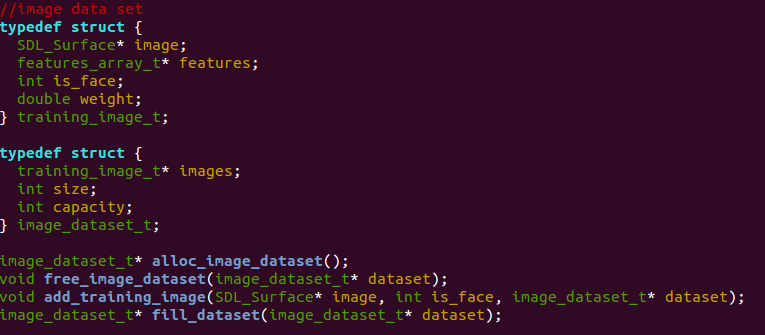
\includegraphics[scale=.5]{Pictures/sdl2.png}
\vspace{0.8cm}

\newpage
\subsection{La base de données}
La base de donnée a été créé en SQLite. Nous pouvons l'utiliser basiquement pour l'instant. La base de donnée a été créé de façon a attribuer un unique identifiant à chaque personne. Nous pouvons actuellement créé la base de donnée, insérer un couple de valeur (Nom d'une personne et sa photo d'identité), supprimer un couple de valeur, afficher la base de donnée dans la console, tout supprimer.

\subsubsection{La création}
La fonction \verb| create_db() | permet de créé la base de donnée avec la table Facificator. Pour l'instant sont créés : Name, Path. Path est le chemin relatif de l'image. D'autres champs seront créés selon notre besoin à venir.

\subsubsection{L'insertion}
La fonction \verb| int insert(char *name, char *image) | permet pour l'instant d'insérer le nom d'une personne et sa photo d'identité. La photo d'identité doit être au préalable stocker dans Database\_Pictures. Nous avons mis au point une fonction pour simplifié la copie de l'image, l'image doit être donnée en paramètre, dans ce dossier. Nous avons fait cela pour des raison évidente de conflit entre chemin absolu sur les différents ordinateur.
\subsubsection{La suppression}
La fonction \verb| delete_id_db(char *id) | permet de supprimer une personne avec toutes les données associées. Pour faire cela nous avons juste besoin de mettre en paramètre l'id que la base de donnée à attribuer la base de donnée. Il faut savoir que l'id restera en "position" occupé.
\subsubsection{L'affichage}
La fonction \verb| create_db() | permet d'afficher la base de donnée dans la console pour pouvoir avoir un visuel.
\subsubsection{La destruction de la base}
La fonction \verb| int destroy_db()| permet de supprimer toute les données que la base contient actuellement, cependant les id ne seront pas réinitialisé.
\subsubsection{L'insertion en masse}
La fonction \verb| int insert_folder (char *folder) | permet d'insérer de multiples personnes dans la base de donnée. Elle prends en paramètre le chemin absolu du dossier où ce trouve toutes les images. Les images seront ensuite copié dans notre dossier d'images. Les images devront porter le nom de la personne. La fonction va donc copier la première image et ensuite appelé la fonction insert avec le nom de l'image et le chemin de l'image copier. Elle réitérera ceci jusqu'à ce qu'elle est traité tout les fichiers.


\newpage
\subsection{La méthode de Viola et Jones}
La méthode de Viola et Jones est basé sur un apprentissage supervisé. Des exemples d'objets doivent être analysés à l'avancé afin d'être classifiés. Ensuite, pendant l'analyse de l'image, des caractéristiques sont choisies par boosting ce qui permet de classifier les caractéristiques, et de séparer les exemples positifs des exemples négatifs par cascade de décision.

Nous avons choisi cette méthode car elle nous parait la plus pratique à mettre en œuvre et la plus optimisée.

\subsubsection{L'image intégrale}
La notion d'image intégrale permet de définir plusieurs zones rectangulaires au sein d'une image. L'intérêt de cette technique est qu'elle offre la possibilité d'accéder à la valeur des autres zones à gauche et au-dessus de la zone sur laquelle nous sommes. Ces zones permettent de créer des caractéristiques pseudo-Haar, qui sont en fait des masques permettant de déterminer plusieurs pattern. 

L'image intégrale est utilisée comme un moyen rapide et efficace de calculer la somme des valeurs (valeurs de pixel) dans une image donnée.
Si l'on souhaite utiliser l'image intégrale, il est préférable de s'assurer d'abord que l'image est en niveaux de gris.
Quand on créé une image intégrale, on a besoin de créer un tableau. Dans ce tableau, en prenant n'importe quel point (x, y), on aura une certaine valeur. Cette valeur est la somme de toutes les valeurs de pixel de gauche, de dessus et bien évidemment, la valeur de pixel d'origine (x, y).

\begin{center}
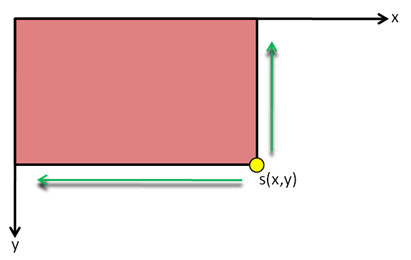
\includegraphics[scale=.7]{Pictures/integrale1.png}
\end{center}

Le tableau peut être construit avec seulement un passage sur l'image donnée. En effet, chaque valeur du tableau est calculée grâce à l'équation suivante : 

\begin{center}

\includegraphics[scale=.7]{Pictures/integrale2.png}
\end{center}

Cette équation signifie que l'on prend la valeur de pixel d'origine, puis on ajoute les valeurs se trouvant sur sa gauche avec s(x-1, y) puis ceux se trouvant au-dessus avec s(x, y-1) et enfin, on soustrait la valeur se trouvant au-dessus à gauche de la valeur de pixel d'origine avec s(x-1, y-1).

Voici un exemple concret d'un calcul :

\begin{center}
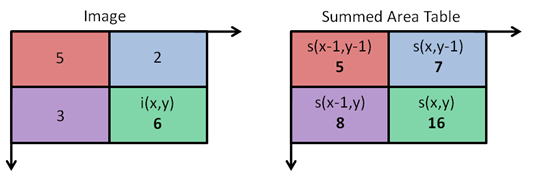
\includegraphics[scale=.7]{Pictures/integrale3.png}
\end{center}

Une fois que nous avons réussi à remplir le tableau, on peut aisément calculer n'importe quel sous-ensemble de l'image originale. Pour cela, il suffit simplement  d'utiliser quatre valeurs du tableau. Avec ces quatre valeurs, on peut les additionner ou les soustraire entre eux afin d'obtenir la bonne valeur de pixel que l'on recherche. On utilise ainsi l'équation suivante :

\begin{center}
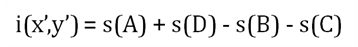
\includegraphics[scale=.7]{Pictures/integrale4.png}
\end{center}

Voici un exemple :
 
\begin{center}
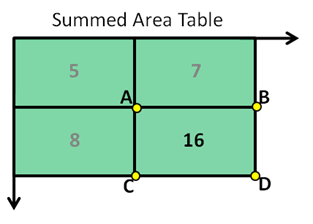
\includegraphics[scale=.7]{Pictures/integrale5.png}
\end{center}

En utilisant l'équation, notre résultat devrait être égal à 6, ce qui est le cas, avec A = 5, B = 7, C = 8 et D = 16.

Pour cette soutenance, nous sommes capable de calculer l'image intégrale de n'importe quelle image et de la stocker dans une matrice. Les calculs de l'image integrale se situe dans pixel\_operations.c et la structure integral\_image contenant le champ int** integral\_image (une matrice de la taille de l'image d'origine) se situe dans types.h.

 \newpage
\subsubsection{Les caractéristiques pseudo-Haar}
Les caractéristiques pseudo-Haar permettent de détecter des motifs. Par exemple, la reconnaissance des visages est rendue possible par exemple par la variation de l'intensité de la lumière entre les yeux et le nez ou la variation de l'intensité de la lumière entre les yeux et les pommettes. 
La méthode de Viola et Jones repose donc sur l'utilisation de ces caractéristiques pseudo-Haar et des images intégrales, améliorant ainsi la vitesse de traitement.

Pour cette soutenance, nous pouvons calculer l'ensemble des caractéristiques de n'importe quelle image de 24 x 24 pixels. Il y a 162 336 caractéristiques dans une telle image. Nous avons utilisés 5 types de caractéristiques: 3 caractéristiques de ligne et 2 caractéristiques de bord; cela est suffisant pour la reconnaissance faciale.

\begin{center}
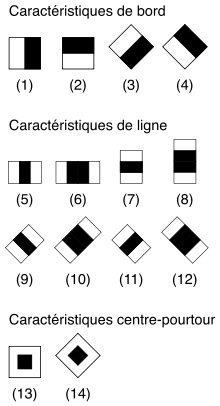
\includegraphics[scale=.7]{Pictures/caracteristiques.png}
\end{center}

\newpage
Le calcul de ces caractéristiques se situe dans pixel\_operations.c et nous nous sommes aidés de cet algorithme :
\newline
\vspace{0.8cm}
\begin{center}
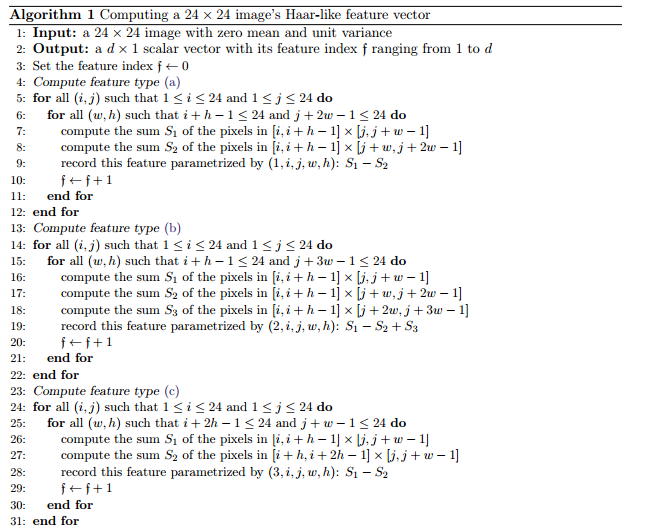
\includegraphics[scale=.7]{Pictures/ipol.png}
\end{center}

\newpage
\subsubsection{L'apprentissage et la classification}
Le classifieur permet de déterminer l'ensemble des zones rentrant sous la coupe d'une caractéristique pseudo-Haar, en déterminant les seuils pouvant déterminer les exemples positifs des négatifs. Ceci demande donc une phase d'apprentissage, qui permet de définir les seuils utilisés. Ensuite, un classifieur est une association entre une caractéristique pseudo-Haar et un seuil. Il existe plusieurs méthodes de boosting (apprentissage et classification) et pour notre projet nous avons choisi Adaboost car elle est très recommandée par sa simplicité a être codée.
\vspace{0.8cm}
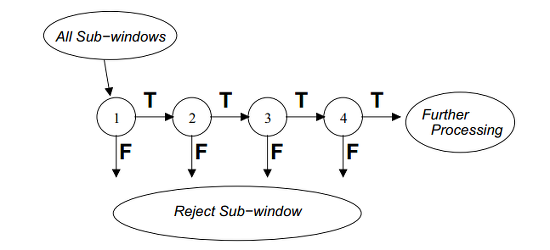
\includegraphics[scale=1]{Pictures/principe-cascade.png}

\newpage
\subsubsection{Adaboost}
Adaboost repose sur la sélection itérative de classifieurs faibles en fonction d'une distribution des exemples d'apprentissage. Chaque exemple est pondéré en fonction de sa difficulté avec le classifieur courant. Ensuite, la somme des classifieurs faibles et d'une constante (alpha dans notre code), calculée à partir de l'erreur minimale, nous donne le classifieur fort. Ce classifieur fort retourne 1 si l'image (24x24)est un visage et 0 sinon.

Nous utilisons une base d'apprentissage de 5000 images contenant un visage et de 5000 images ne contenant pas de visages (ce sont des training\_image\_t dans notre code). Ces images sont toutes de taille 24x24 pixels et sont en nuances de gris. La structure image\_dataset\_t (types.h) contiendra toutes ces training\_image\_t.

Notre Adaboost est capable de calculer les seuils pouvant déterminer les exemples positifs et négatifs; il calcule T classifieurs faibles, avec, pour chacun, l'erreur la plus minimale possible. Toutes les fonctions concernant Adaboost (que ce soit l'apprentissage ou la classification) se trouve dans le fichier adaboost.c.
Nous avons utilise le multi-coeur pour l'apprentissage final. Ce qui a permis de faire l'apprentissage 8 fois plus rapidement que la normale car nous avons déployé 8 threads (une thread par coeur) lors de la sélection des caractéristiques.

\vspace{0.8cm}
\begin{center}
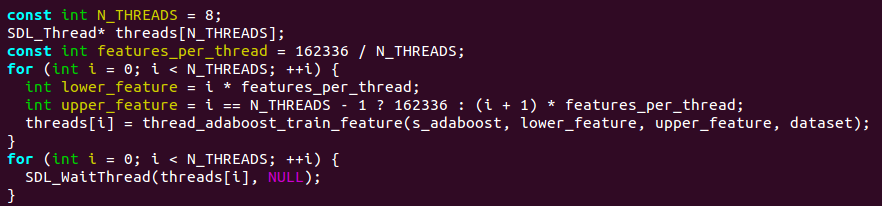
\includegraphics[scale=.5]{Pictures/threads.png}
\end{center}

\newpage
Nous nous sommes aider de cet algorithme pour réaliser notre version d'Adaboost en C :

\vspace{0.8cm}
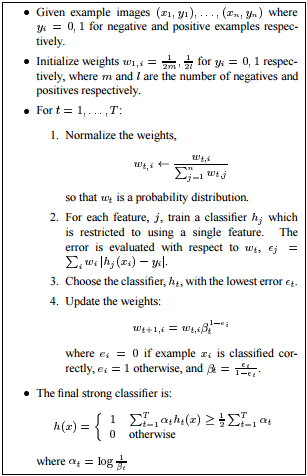
\includegraphics[scale=1]{Pictures/adaboost.png}

\newpage
Voici des exemples de caractéristiques intéressantes que notre Adaboost a sélectionne :

\vspace{0.8cm}
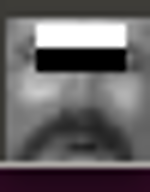
\includegraphics[scale=.5]{Pictures/feature5.png}
\newline
Les yeux sont plus sombres que le front.

\vspace{0.8cm}

\includegraphics[scale=.5]{Pictures/feature4.png}
\newline
Le nez est plus clair que les yeux.

\vspace{0.8cm}
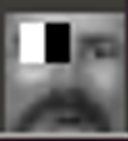
\includegraphics[scale=.5]{Pictures/feature3.png}
\newline
Encore une fois la différence entre le nez et l'œil droit.

\vspace{0.8cm}
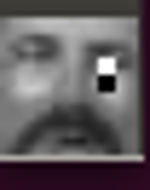
\includegraphics[scale=.5]{Pictures/feature2.png}
\newline
L'œil est souvent plus sombre que la joue.

\vspace{0.8cm}
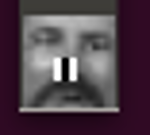
\includegraphics[scale=.5]{Pictures/feature1.png}
\newline
La barbe est également une caractéristique intéressante qui est plus sombre que le nez et la bouche.

\newpage
\subsubsection{La cascade de classifieurs}
Nous nous sommes aider de cet algorithme pour réaliser notre cascade de classifieurs en C:
\vspace{0.8cm}
\newline
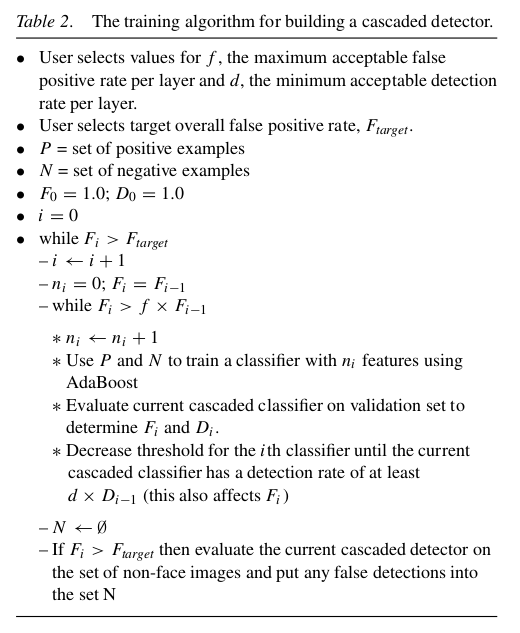
\includegraphics[scale=.7]{Pictures/cascade.png}

\newpage
La cascade finale possède 10 niveaux de 2, 5, 10, 20, 25, 25, 30, 40, 50 et 60 classifieurs forts. 

Voici le fichier qui contient notre cascade de classifieurs :
\vspace{0.8cm}
\begin{center}
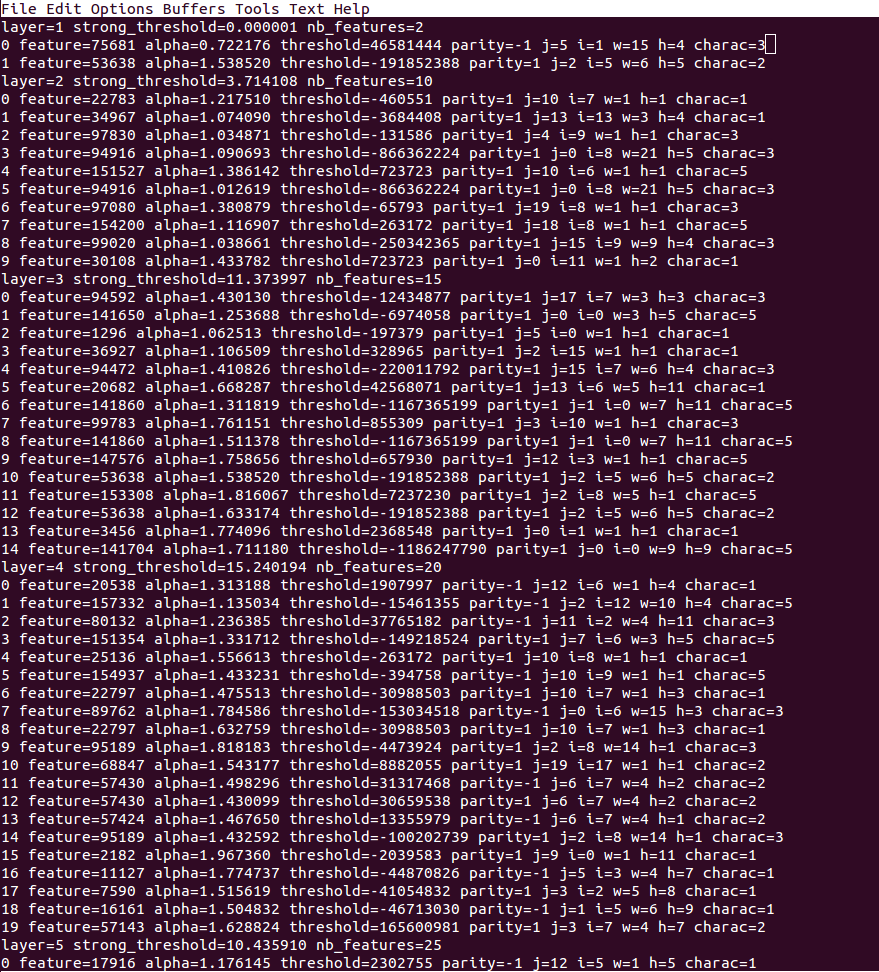
\includegraphics[scale=.4]{Pictures/cascade-file.png}
\end{center}


\newpage
\subsubsection{La détection}

Voila le résultat de notre première cascade sur une photo de l'équipe de France de football :
\vspace{0.8cm}
\newline
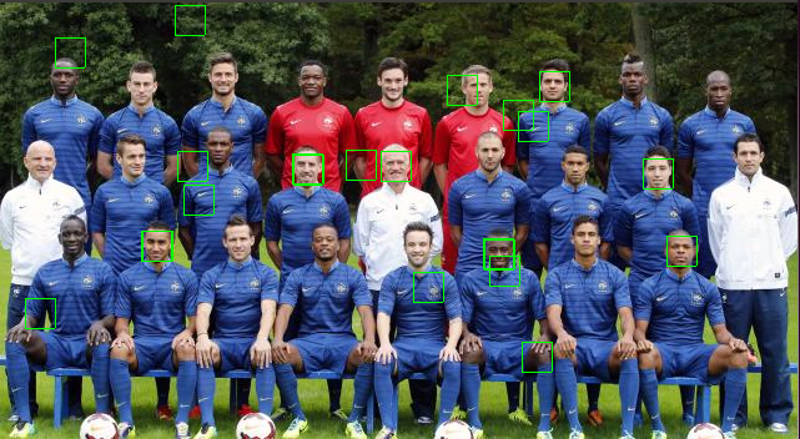
\includegraphics[scale=0.5]{Pictures/france.png}

\vspace{0.8cm}
Nous voyons que quelques visages sont détectés mais il y a encore des "faux positifs", c'est-a-dire des non visages qui sont encadres.

\vspace{0.8cm}
Après 12 heures d'apprentissage et plusieurs versions d'adaboost et de cascade, nous avons obtenu une détection très fiable de visages vus de face.
\vspace{0.8cm}
\begin{center}
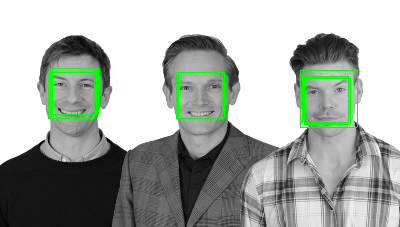
\includegraphics[scale=0.5]{Pictures/detection.png}
\end{center}


\newpage
Voici a présent la différence de détection avec 5, 8 et 10 niveaux de notre cascade finale :
\begin{center}
\vspace{0.8cm}
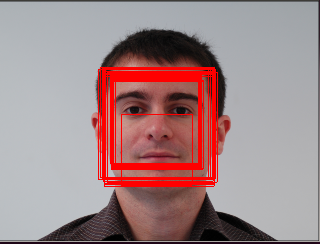
\includegraphics[scale=0.5]{Pictures/frontal_5layers.png}
\vspace{0.8cm}
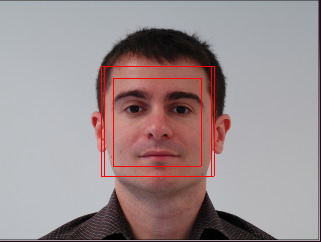
\includegraphics[scale=0.5]{Pictures/frontal_8layers.png}
\vspace{0.8cm}
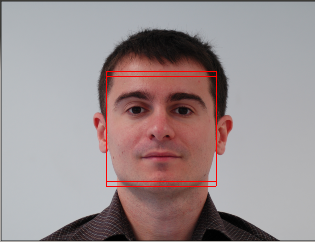
\includegraphics[scale=0.5]{Pictures/frontal_10layers.png}
\end{center}

Nous remarquons que plus il y a de niveaux, plus la détection va être précise.

\newpage
\subsection{Les eigenfaces}

	Alors que la détection de visage est mis en place la suite logique et leurs reconnaissance. Afin de reconnaitre ces visage plusieurs calcul sont a effectuer afin de déterminer si oui ou non un visage soumit appartient a une base de donnée. mais avant de commencer les calcul en eux même il faut effectuer un pretraitement de l'image.

\subsubsection{Pré traitement}
	
	Le pré traitement vise en le redimensionnement, l'égalisation et la normalisation de l'image afin de permettre une cohérence des résultats de calculs sur tout visage soumis au logiciels. Chaque visage est soumis au logiciel sous forme de matrice des pixels qui le compose.\\


\begin{itemize}
	
\item Redimensionnement : Vise à rogner l'image dans une taille standard afin de rendre possible certains calculs\\

\item Normalisation : La normalisation consiste à améliorer le contraste d'une image à partir de son histogramme. Cela consiste à repartir de manière équitable les nuances de gris sur la globalité de l'image 
exemple: \\
\begin{center}
\vspace{0.8cm}
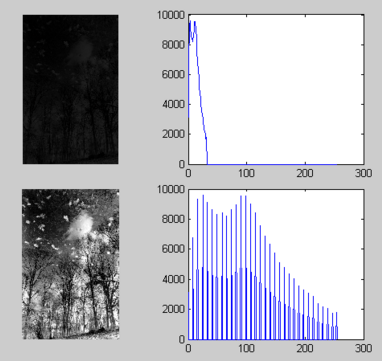
\includegraphics[scale=0.5]{Pictures/normalisation.png} 
\end{center}


Sur l'ordonnée on constate l'intensité du niveau de gris et en abscisse le nombre de pixel possédant une nuance en particulière ainsi une meilleure répartition horizontale améliore le contraste.\\

\item L'égalisation : Consiste à réduire la différence d'amplitude entre les niveaux de gris\\

\end{itemize}

\subsubsection{Matrice de covariance et valeurs propres}


Maintenant que les visage sont pretraités les calculs d'identification peuvent commencer. Ainsi la première étage consiste à calculer un visage moyen à partir de l'ensemble des visages contenus dans la base de données. ce visage G est calculé par \[ G = \frac{1}{N}\sum_{k=1}^{N} V_{i}\]  avec N le nombre de visage de la base de donne et V un visage de celle ci\\
A partir de ce visage générique on calcule la différence entre chaque visage et le visage moyen. Notons T ce vecteur. Les calculs sont les suivants . \[ U_{i} = V_{i} - G\] \[ T = \{ U_{1}, U_{2}, ..., U_{N}\}\]\\
A partir de ce vecteur nous pouvont créer une matrice A en concaténant chaque élément de celui-ci. Ensuite il nous faut calculer la matrice de covariance C donner par la formule suivante \[ C = AA^{t} \] Cette matrice de covariance nous permet de calculer une valeur propre P grâce à la limite suivante \[P =\lim_{n \to +\infty} W_ {n}\] \[W_{n} = \frac{C^{n} * X }{| C^{n} *X |}\]
Ou X est un vecteur colonne arbitraire de même taille que C \\\\  Cette valeur propre sera comparer à celle de l'image à analyser et si elle sont similaire cela signifie que le visage appartiendra la base de données. La similarité est déterminée par un seuil d'erreur définis arbitrairement.

\newpage
\subsection{L'interface graphique}
L'interface graphique permet un contrôle du programme de manière beaucoup plus intuitive que du simple code. Ce qui est d'une grande importance étant donné que toute la population n'est pas experte en informatique. Ainsi le développement d'une interface graphique permet à de potentiels clients ou collaborateurs d'exploiter le programme sans avoir à passer une formation spécialisée. 

\subsubsection{La programmation événementiel}
L'interface graphique permet le déclenchement d'événements en fonction de l'utilisateur. Or, la programmation classique, c'est-à-dire l'exécution d'algorithmes de manière séquentielle, ne permet pas ce genre d'interactions.  C'est pourquoi une nouvelle philosophie de programmation a vu le jour. Tout comme la programmation orientée objet, la programmation événementielle possède ses propres règles.

La structure se décompose en une boucle générale dans laquelle toutes les possibilités d'actions de l'utilisateur sont prises en compte dans laquelle se trouvent différents modules. Dans cette boucle plusieurs modules, appelés widgets ("chose" en anglais), sont définis. Ces widgets permettent l'affichage de différentes fenêtres, boutons, textes etc.
Pour que l'utilisateur puisse interagir avec les différentes fenêtres définies plus tôt, une nouvelle notion devra être intégrée : les fonctions callback. Ces fonctions ont un but très simple : déclencher un événement (ouverture d'une fenêtre, affichage de texte etc.) lorsque l'utilisateur effectue une action précise (survole avec le curseur, clique sur un bouton). Pour effectuer cette tâche, les fonctions callback possèdent toutes la même structure, trois paramètres : un widget, une action et une fonction. Le paramètre widget sert a indiquer quel objet devra subir l'action pour déclencher l'événement, le paramètre action définit le type d'action (clique, survole...) et enfin le dernier paramètre est une fonction. Cette fonction décrit l'ensemble des instructions à effectuer si l'action est réalisée.

La combinaison des widgets et des fonctions callback permettent la création d'une interface graphique très complète et modulable à souhait.

\subsubsection{La forme}

\includegraphics[scale=0.3]{Pictures/interface.png} 

L'interface graphique contient tout d'abord une barre de menu contenant 4 sous-menus, "Fichier", "Édition", "Base de donnée" et "Aide" et un cadre affichant une image de base. Mais également quatre boutons, "Charger une image", "Détection", "Ajout" et "Suppression". 
\newline

\begin{center}
\includegraphics[scale=1]{Pictures/bouton_interface.png} 
\end{center}
% Image de la barre de menu
% Image des 4 boutons

\subsubsection{Le fond}

Pour chacun des boutons, le signal "clicked" a été associé à une fonction spécifique.
Concernant le bouton "Charger une image", lorsque l'on clique sur le bouton, la fonction qui a été connecté à ce bouton, grâce au signal "clicked", permet d'afficher une nouvelle fenêtre. Cette nouvelle fenêtre contient un bouton permettant de sélectionner l'image que l'on souhaite et de l'afficher sur la fenêtre principale tout en fermant la fenêtre secondaire qui avait été ouverte.
\begin{center}
\includegraphics[scale=1]{Pictures/interface2.png} \\
\includegraphics[scale=0.7]{Pictures/interface3.png} \\
\includegraphics[scale=0.9]{Pictures/interface4.png} \\

\end{center}

Concernant le bouton "Détection", lorsque l'on clique sur le bouton, la fonction qui a été connecté à ce bouton, grâce au signal "clicked" aussi, va lancer l'algorithme adaboost, qui va ainsi permettre de lancer la détection de visage sur l'image que l'on aura au préalable charger grâce au bouton présenté précédemment.
%Image après adaboost fini

Concernant le bouton "Ajout", lorsque l'on clique sur le bouton, la fonction qui a été connecté à ce bouton, grâce au signal "clicked", permet d'afficher une nouvelle fenêtre \\
\begin{center}
\includegraphics[scale=1]{Pictures/interface5.png} 
\end{center}


\newpage
\section{Conclusion}
Les premières semaines de projet avaient été très motivantes. Toutes les difficultés que nous avions rencontrées avaient été surmonté. De plus, nous avions réussi à respecter notre planning, voir sur certaines parties nous avions pris une légère avance. Nous espérions garder cette avance pour pouvoir surmonter toutes les difficultés qui nous attendaient. Cependant, l'avance pris après la première soutenance fut très vite dissiper. En effet, il s'avère que le projet fut beaucoup plus difficile que ce que nous pensions. Mais nous sommes malgré la difficulté parvenus à obtenir un logiciel permettant la reconnaissance de visage dans une photo, c'est-à-dire de nous indiquer si un visage est présent ou non sur une photo.
Malgré que le projet ne soit pas totalement fini car, les objectifs n'ont pas été tous atteint, nous pouvons dire que nous sommes assez fier du logiciel que nous avons obtenu.

\end{document}
